% ECE501 Digital Image Processing -- Week 7 Project Progress Report (Group 15)
% Build: tectonic main.tex
\documentclass[11pt,a4paper]{article}

\usepackage[margin=2.2cm]{geometry}
\usepackage[T1]{fontenc}
\usepackage{lmodern}
\usepackage{microtype}
\usepackage{amsmath,amssymb}
\usepackage{graphicx}
\usepackage{booktabs}
\usepackage{tabularx}
\usepackage{longtable}
\usepackage{array}
\usepackage{multirow}
\usepackage[table]{xcolor}
\usepackage{enumitem}
\usepackage{caption}
\usepackage{fancyhdr}
\usepackage{listings}
\usepackage{tikz}
\usepackage{placeins}
\usetikzlibrary{positioning,arrows.meta,fit,backgrounds}
\usepackage[colorlinks=true,linkcolor=blue!50!black,citecolor=blue!60!black,urlcolor=blue!60!black]{hyperref}

\definecolor{hdr}{HTML}{DCE6F2}
\definecolor{codebg}{HTML}{F6F8FA}
\definecolor{okgreen}{HTML}{1E7B34}
\definecolor{badred}{HTML}{B3261E}

\newcommand{\code}[1]{\texttt{\detokenize{#1}}}
\newcolumntype{L}{>{\raggedright\arraybackslash}X}
\newcolumntype{C}{>{\centering\arraybackslash}X}
\newcolumntype{R}{>{\raggedleft\arraybackslash}X}

\lstset{
  basicstyle=\ttfamily\footnotesize,
  backgroundcolor=\color{codebg},
  frame=single, rulecolor=\color{black!15},
  breaklines=true, columns=fullflexible,
  keywordstyle=\color{blue!60!black}\bfseries,
  commentstyle=\color{black!55}\itshape,
  stringstyle=\color{okgreen},
  showstringspaces=false,
  xleftmargin=2pt, xrightmargin=2pt
}

\captionsetup{font=small,labelfont=bf}
\setlist{itemsep=2pt,topsep=4pt}
\emergencystretch=3em

\pagestyle{fancy}
\fancyhf{}
\fancyfoot[C]{\small Group 15 \textbar\ Week 7 Project Progress Report \textbar\ Page \thepage}
\renewcommand{\headrulewidth}{0pt}

\begin{document}

\begin{center}
{\LARGE\bfseries Week 7 Project Progress Report}\\[4pt]
{\large\bfseries Adaptive Fabric Surface Defect Detection and Localization using\\ Classical Texture Descriptors}
\end{center}

\noindent
\textbf{Course Name:} ECE501 Digital Image Processing (DIP)\\
\textbf{Group Number:} Group 15\\
\textbf{Group Members:} Rinal Shah, Varun Hotani, Aadi Mehta, Pratik Agrawal\\
\textbf{Week Number:} Week 7\\
\textbf{Date:} October 31, 2026\\
\textbf{Deliverable:} Image-level detection with a calibrated confidence score; cross-validated in-domain reference against the AFID capture shift; $64\rightarrow32$ refinement cascade; small-defect protocol study; frozen evaluation protocol\\
\textbf{Branch:} \code{feat/week-7} (merged into \code{main})

\section*{Objectives of the Week}
The Week~6 report ended with four items for this week. Each is addressed here:
\begin{itemize}
  \item \textbf{Image-level detection and confidence.} Hold out defect-free strips as true negatives, decide per strip whether it is defective, and attach a confidence with a provable false-alarm guarantee.
  \item \textbf{Capture shift.} Use the defect-free \emph{regions} of defective strips as extra reference data. Cross-validate by strip, so that no strip is ever scored by a model that saw any of its pixels.
  \item \textbf{Small defects.} Add a $32\times32$ level to the refinement cascade, and measure how the 25-pixel patch-label rule hides the smallest defects.
  \item \textbf{End-semester preparation.} Freeze the evaluation protocol and make every reported table regenerate from committed results.
\end{itemize}

\section*{Summary of the Week}
\begin{center}
\renewcommand{\arraystretch}{1.15}
\begin{tabularx}{\textwidth}{@{}lL@{}}
\toprule
\textbf{Item} & \textbf{Outcome} \\
\midrule
Protocol & Per fabric, the 20 defect-free strips split by image (seeded): 12 fit, 4 calibrate, 4 held-out negatives. 105 defective + 28 defect-free test strips \\
Image level & Accuracy \textbf{68.42\,\%}, detection rate 60.00\,\%, \textbf{zero false alarms} on the 28 negatives ($\alpha=0.05$), AUROC \textbf{0.790} \\
Localization & Unchanged by the new protocol: patch F1 18.38\,\% (pooled 23.02\,\%), pixel IoU 1.36\,\%, pixel recall 48.41\,\% \\
Threshold-free diagnosis & New per-strip \emph{window AUROC}: 0.536 for the default, 0.609 with the in-domain reference. The descriptors rank defect windows only slightly better than chance within a strip. \\
In-domain reference & Raises window AUROC (broken ends 0.12 $\rightarrow$ 0.69) but over-tightens $\tau$: pixel recall 48\,\% $\rightarrow$ 11\,\%. Kept as an option, not the default. \\
Small defects & $64\rightarrow32$ cascade: pixel IoU 1.36 $\rightarrow$ 1.52\,\%. ``Any defect pixel'' labels: warp balls measurable for the first time (window AUROC 0.826) \\
Quality & 86 tests (72 last week); every table in this report is generated from \code{Results/} by \code{reports/week-7/make_tables.py} \\
\bottomrule
\end{tabularx}
\end{center}

%=====================================================================
\section*{Work Completed This Week}

\subsection*{A. A Frozen, Three-Way Evaluation Protocol}

Until Week~6 every test strip was defective. That measures localization, but it cannot measure what an inspection line needs first: \emph{whether a roll segment should be stopped at all}. Each fabric's 20 defect-free strips are now split \emph{by strip} with a seeded permutation into three disjoint sets:
\begin{equation}
\underbrace{12}_{\text{fit }\boldsymbol{\mu}_f,\boldsymbol{\Sigma}_f}\;+\;\underbrace{4}_{\text{calibrate }\tau_f\text{, confidence}}\;+\;\underbrace{4}_{\text{image-level negatives}}
\label{eq:split}
\end{equation}
(\code{calibration_fraction} $=$ \code{test_fraction} $=0.2$). The test set is therefore 105 defective strips (every one with a mask and a reference fabric) plus 28 defect-free strips, none of which touches fitting or calibration. Patch and pixel metrics are still computed on defective strips only; image-level metrics use all 133. Moving from 15 to 12 fit strips changed the localization results by less than 0.3 percentage points (patch F1 18.14 $\rightarrow$ 18.38\,\%, IoU 1.36\,\% both weeks).

\subsection*{B. Image-Level Decision and Conformal Confidence}

\paragraph{Image score.} A strip is as anomalous as its most anomalous window, measured in units of its fabric's threshold:
\begin{equation}
S=\frac{\max_i s_i}{\tau_f}\qquad(S\ge1\iff\text{at least one window is flagged}).
\label{eq:imgscore}
\end{equation}
Dividing by $\tau_f$ puts all seven fabrics on one scale, so one calibration set can serve all of them.

\paragraph{Confidence.} We use a conformal p-value \cite{vovk2005,laxhammar2015}. Let $S_1,\dots,S_n$ be the image scores of the $n=28$ held-out \emph{calibration} strips (4 per fabric, never fitted on). For a test strip with score $S$,
\begin{equation}
p(S)=\frac{1+\#\{j: S_j\ge S\}}{n+1},\qquad \text{confidence}=1-p(S),\qquad \text{defective}\iff p(S)\le\alpha .
\label{eq:conformal}
\end{equation}
If defect-free test strips are exchangeable with the calibration strips (same capture, same distribution), then $\Pr[p\le\alpha]\le\alpha$. The false-alarm rate is bounded by $\alpha$ without any assumption on the score distribution. With $n=28$ the smallest attainable p-value is $1/29\approx0.034$, so $\alpha=0.05$ means ``more anomalous than every calibration strip''. A unit test checks the bound empirically: 5{,}000 exchangeable draws against 199 calibration scores give a flagged rate of at most 6\,\% at $\alpha=0.05$.

\subsection*{C. Cross-Validated In-Domain Reference}

Week~6 showed that normal windows of defective strips score far above held-out \emph{defect-free} strips for five fabrics, a capture shift between AFID's two image sets. The natural fix is to learn ``normal'' from the same capture: the windows of defective strips that contain \emph{no} defect pixel. Doing this naively leaks test information, so \code{model.reference = "in_domain"} runs a strip-level cross-validation:
\begin{enumerate}
  \item Per fabric, the defective strips are shuffled (seeded) and dealt into $K=\min(5,n_f)$ folds; that fabric's negatives are dealt round-robin into the same folds.
  \item For fold $j$, the training strips are the fabric's defective strips \emph{outside} fold $j$. They are split again by strip into an inner fit part and an inner calibration part (20\,\%).
  \item The reference is fitted on the defect-free fit strips \emph{plus} the zero-defect windows of the inner-fit training strips. $\tau_f$ and the conformal calibration use the defect-free calibration strips \emph{plus} the zero-defect windows of the inner-calibration strips. This is done at $256\times256$ and at every refinement level.
  \item Fold $j$'s strips are then scored. Every strip is scored exactly once, by a model that never saw any of its windows.
\end{enumerate}
A window counts as defect-free when its summed-area-table count of mask pixels is exactly 0. Fabric 05 has a single defective strip, so there is nothing to learn from; it keeps the defect-free reference. The fold assignment, the inner split and the background selection are covered by unit tests.

\subsection*{D. Refinement Cascade}

\code{refine.sizes} replaces Week~6's single fine level with a coarse-to-fine list, e.g.\ $[64,32]$ (stride $=$ size$/2$). The windows flagged at one level bound the next:
\begin{equation}
R_0=\bigcup_{w\in\mathcal{F}_{256}}w,\qquad
R_{\ell}=\bigcup\big\{v\in\mathcal{V}_{s_\ell}: v\subseteq R_{\ell-1},\ d^{(s_\ell)}_f(\mathbf{x}_v)\ge\tau^{(s_\ell)}_f\big\},\qquad \hat M=\mathrm{morph}(R_L),
\label{eq:cascade}
\end{equation}
with one Mahalanobis reference and one held-out $\tau$ per fabric and level. The $32\times32$ level needs about 3{,}700 windows per strip, so it was added to the feature cache once (about 12 minutes for all 246 strips on 8 processes); every later run reuses it.

\subsection*{E. Threshold-Free Window AUROC}

All earlier patch metrics depend on $\tau$. To separate ``the descriptor cannot tell defect from background'' from ``the threshold is in the wrong place'', each defective strip now also reports the AUROC of its window scores against its window labels:
\begin{equation}
\mathrm{AUROC}_{\text{strip}}=\Pr\big[s_i>s_j \mid i\text{ defect window},\ j\text{ normal window of the same strip}\big],
\label{eq:wauroc}
\end{equation}
averaged over strips that have both kinds of window. 0.5 is chance; values below 0.5 mean the defect scores \emph{lower} than its surroundings.

%=====================================================================
\section*{Quantitative Results and Analysis}

All numbers are on \textbf{real AFID data}, with seed 0 and the protocol of Eq.~\eqref{eq:split}: 105 defective strips for patch and pixel metrics, plus 28 defect-free strips for image-level metrics. Tables~\ref{tab:ablation}--\ref{tab:defect} are generated from \code{Results/final/} and \code{Results/ablation/}.

\begin{table}[h]
\centering
\caption{Ablation (one factor at a time around the default; \%, except AUROC). Patch/pixel columns: 105 defective strips. Image columns: the same plus 28 defect-free strips.}
\label{tab:ablation}
\scriptsize
\setlength{\tabcolsep}{2.4pt}
\begin{tabularx}{\textwidth}{@{}>{\raggedright\arraybackslash}p{0.24\textwidth}RRRRRRRRR@{}}
\toprule
& \multicolumn{5}{c}{\textbf{Localization (defective strips)}} & \multicolumn{4}{c}{\textbf{Image level}} \\
\cmidrule(lr){2-6}\cmidrule(l){7-10}
\textbf{Variant} & \textbf{Patch F1} & \textbf{Pooled F1} & \textbf{Win.\ AUROC} & \textbf{IoU} & \textbf{Pix.\ rec.} & \textbf{Acc.} & \textbf{Det.\ rate} & \textbf{Spec.} & \textbf{AUROC} \\
\midrule
\textbf{default} & 18.38 & 23.02 & 0.536 & 1.36 & 48.41 & 68.42 & 60.00 & 100.00 & 0.790 \\
features: glcm & 18.18 & 22.59 & 0.529 & 1.38 & 49.10 & 69.17 & 60.95 & 100.00 & 0.792 \\
features: lbp & 12.76 & 21.74 & 0.458 & 1.13 & 39.58 & 63.16 & 54.29 & 96.43 & 0.796 \\
features: gabor & 15.81 & 22.69 & 0.529 & 0.89 & 56.58 & 72.93 & 65.71 & 100.00 & 0.878 \\
features: glcm+\allowbreak{}lbp+\allowbreak{}gabor & 16.49 & 22.64 & 0.540 & 1.05 & 57.73 & 70.68 & 62.86 & 100.00 & 0.853 \\
scoring: strip mahalanobis & 8.16 & 12.34 & 0.546 & 0.46 & 7.01 & 33.83 & 17.14 & 96.43 & 0.366 \\
scoring: hybrid (week 5) & 14.01 & 14.85 & 0.574 & 0.71 & 26.76 & 49.62 & 36.19 & 100.00 & 0.675 \\
scoring: relative & 14.57 & 16.57 & 0.551 & 0.87 & 29.99 & 48.12 & 34.29 & 100.00 & 0.689 \\
baseline: one-class svm & 16.71 & 23.43 & 0.572 & 1.32 & 43.70 & 61.65 & 55.24 & 85.71 & 0.697 \\
baseline: isolation forest & 14.40 & 18.68 & 0.616 & 0.95 & 40.13 & 47.37 & 33.33 & 100.00 & 0.669 \\
reference: global (fixed) & 5.77 & 12.02 & 0.461 & 0.08 & 22.82 & 42.11 & 26.67 & 100.00 & 0.744 \\
reference: in-domain (cross-validated) & 7.86 & 12.54 & 0.609 & 0.35 & 10.60 & 45.11 & 30.48 & 100.00 & 0.736 \\
k = 2.0 & 18.82 & 23.23 & 0.536 & 1.41 & 50.41 & 69.17 & 60.95 & 100.00 & 0.789 \\
k = 3.0 & 18.60 & 22.40 & 0.536 & 1.37 & 46.98 & 68.42 & 60.00 & 100.00 & 0.792 \\
refine: off & 18.38 & 23.02 & 0.536 & 0.71 & 54.93 & 68.42 & 60.00 & 100.00 & 0.790 \\
refine: 64 then 32 & 18.38 & 23.02 & 0.536 & 1.52 & 43.75 & 68.42 & 60.00 & 100.00 & 0.790 \\
refine: 32 only & 18.38 & 23.02 & 0.536 & 1.55 & 46.10 & 68.42 & 60.00 & 100.00 & 0.790 \\
patch label: any defect pixel & 19.77 & 24.52 & 0.557 & 1.36 & 48.41 & 68.42 & 60.00 & 100.00 & 0.790 \\
image alpha = 0.10 & 18.38 & 23.02 & 0.536 & 1.36 & 48.41 & 69.92 & 61.90 & 100.00 & 0.790 \\
week 5 setting & 14.01 & 14.85 & 0.574 & 0.30 & 32.88 & 49.62 & 36.19 & 100.00 & 0.675 \\
\bottomrule

\end{tabularx}
\end{table}

\begin{table}[h]
\centering
\caption{Image-level detection per fabric (default, $\alpha=0.05$). Negatives: 4 held-out defect-free strips per fabric.}
\label{tab:imgfabric}
\small
\begin{tabularx}{\textwidth}{@{}lrrRRRR@{}}
\toprule
\textbf{Fabric} & \textbf{Defective} & \textbf{Defect-free} & \textbf{Accuracy} & \textbf{Detection rate} & \textbf{Specificity} & \textbf{AUROC} \\
\midrule
fabric\_00 & 7 & 4 & 72.73 & 57.14 & 100.00 & 0.643 \\
fabric\_01 & 12 & 4 & 100.00 & 100.00 & 100.00 & 1.000 \\
fabric\_02 & 38 & 4 & 66.67 & 63.16 & 100.00 & 0.770 \\
fabric\_03 & 31 & 4 & 71.43 & 67.74 & 100.00 & 0.927 \\
fabric\_04 & 10 & 4 & 28.57 & 0.00 & 100.00 & 0.550 \\
fabric\_05 & 1 & 4 & 100.00 & 100.00 & 100.00 & 1.000 \\
fabric\_06 & 6 & 4 & 50.00 & 16.67 & 100.00 & 1.000 \\
\bottomrule

\end{tabularx}
\end{table}

\begin{table}[h]
\centering
\caption{Default configuration per fabric (defective strips; \%, except window AUROC). ``Detected'' is the image-level detection rate.}
\label{tab:fabric}
\small
\setlength{\tabcolsep}{3pt}
\begin{tabularx}{\textwidth}{@{}lrRRRRRRR@{}}
\toprule
\textbf{Fabric} & $n$ & \textbf{Patch prec.} & \textbf{Patch rec.} & \textbf{Patch F1} & \textbf{Win.\ AUROC} & \textbf{Pixel IoU} & \textbf{Pixel rec.} & \textbf{Detected} \\
\midrule
fabric\_00 & 7 & 7.70 & 71.43 & 13.68 & 0.461 & 0.06 & 57.14 & 57.14 \\
fabric\_01 & 12 & 14.83 & 100.00 & 21.05 & 0.366 & 1.93 & 89.15 & 100.00 \\
fabric\_02 & 38 & 3.92 & 75.00 & 7.20 & 0.483 & 0.09 & 55.26 & 63.16 \\
fabric\_03 & 31 & 38.39 & 62.31 & 33.57 & 0.633 & 3.73 & 39.15 & 67.74 \\
fabric\_04 & 10 & 0.00 & 0.00 & 0.00 & 0.640 & 0.00 & 0.00 & 0.00 \\
fabric\_05 & 1 & 6.90 & 100.00 & 12.90 & 0.074 & 0.03 & 100.00 & 100.00 \\
fabric\_06 & 6 & 25.00 & 30.00 & 25.00 & 0.759 & 0.08 & 31.67 & 16.67 \\
\bottomrule

\end{tabularx}
\end{table}

\begin{table}[h]
\centering
\caption{Default configuration per official defect class (defective strips; \%, except window AUROC). ``--'': undefined (no window holds more than 25 mask pixels).}
\label{tab:defect}
\small
\setlength{\tabcolsep}{3pt}
\begin{tabularx}{\textwidth}{@{}lrRRRRRRR@{}}
\toprule
\textbf{Defect} & $n$ & \textbf{Patch prec.} & \textbf{Patch rec.} & \textbf{Patch F1} & \textbf{Win.\ AUROC} & \textbf{Pixel IoU} & \textbf{Pixel rec.} & \textbf{Detected} \\
\midrule
broken\_end & 9 & 6.53 & 88.89 & 12.14 & 0.121 & 0.11 & 85.66 & 100.00 \\
broken\_pick & 10 & 76.00 & 60.60 & 52.77 & 0.776 & 10.91 & 47.99 & 80.00 \\
broken\_yarn & 8 & 6.91 & 87.50 & 11.30 & 0.278 & 0.12 & 87.50 & 87.50 \\
contamination & 1 & 0.00 & 0.00 & 0.00 & 0.793 & 0.00 & 0.00 & 0.00 \\
crease & 5 & 7.61 & 60.00 & 13.25 & 0.546 & 0.49 & 80.00 & 60.00 \\
cut\_selvage & 9 & 41.93 & 55.56 & 40.42 & 0.864 & 0.22 & 43.34 & 33.33 \\
fuzzy\_ball & 39 & 7.61 & 47.22 & 9.25 & 0.696 & 0.01 & 25.64 & 43.59 \\
knot & 1 & 6.90 & 100.00 & 12.90 & 0.074 & 0.03 & 100.00 & 100.00 \\
nep & 14 & 4.75 & 69.23 & 8.82 & 0.442 & 0.02 & 64.29 & 85.71 \\
warp\_ball & 5 & 0.00 & -- & 0.00 & -- & 0.02 & 20.00 & 0.00 \\
weft\_crack & 1 & 93.55 & 100.00 & 96.67 & 0.328 & 22.39 & 98.83 & 100.00 \\
weft\_curling & 3 & 14.84 & 50.00 & 22.88 & 0.488 & 1.57 & 47.53 & 66.67 \\
\bottomrule

\end{tabularx}
\end{table}

\begin{figure}[h]
\centering
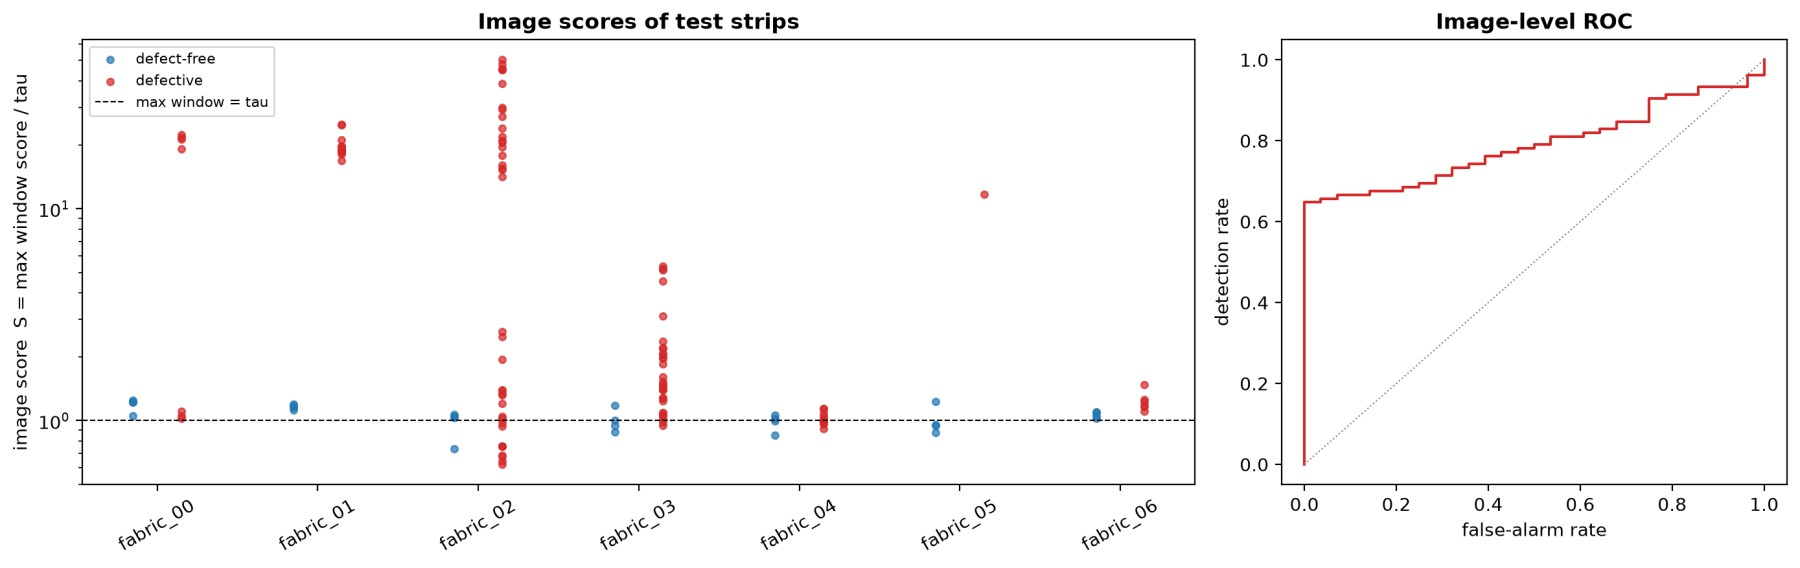
\includegraphics[width=\textwidth]{figures/image_scores.jpg}
\caption{Left: image scores $S$ (Eq.~\ref{eq:imgscore}, log scale) of the 28 held-out defect-free strips (blue) and the 105 defective strips (red), per fabric; the dashed line is $S=1$. Right: image-level ROC over all 133 strips (AUROC 0.790).}
\label{fig:scores}
\end{figure}

%=====================================================================
\FloatBarrier
\section*{Discussion of Findings}
\begin{enumerate}
  \item \textbf{The conformal decision is what makes image-level detection usable.} With the naive rule ``defective if any window crosses $\tau_f$'' ($S\ge1$), 20 of the 28 defect-free test strips would be false alarms, because a 4{,}096-px strip has about 30 windows and each may cross a per-window threshold by chance. The conformal rule (Eq.~\ref{eq:conformal}) instead calibrates the \emph{strip-level} statistic. Its effective cut-off falls between $S=1.34$ and $S=1.38$. It produced no false alarm on the 28 negatives while detecting 63 of 105 defective strips (60.0\,\%), and the threshold-free AUROC is 0.790.
  \item \textbf{Image-level numbers are inflated where AFID's captures differ.} The median image score of defective strips is 8.4--19.2 for fabrics 00, 01, 02 and 05, against 0.95--1.22 for their defect-free test strips (Figure~\ref{fig:scores}). That gap is mostly the capture shift reported in Week~6, not the defect. The fair test is fabrics 03, 04 and 06, whose captures transfer:
  \begin{itemize}
    \item \textbf{Fabric 03:} AUROC 0.927 and 67.7\,\% detection, a real defect signal (broken picks, weft curling).
    \item \textbf{Fabric 06:} AUROC 1.000 but only 16.7\,\% detection.
    \item \textbf{Fabric 04:} its 10 small defects are not separable at all (AUROC 0.550, nothing detected).
  \end{itemize}
  \item \textbf{Within a strip, window scores barely rank defects above background.} The mean window AUROC of the default is 0.536 (Table~\ref{tab:ablation}). For broken ends and knots it is far \emph{below} 0.5: in those shifted fabrics the whole strip is anomalous, and the thin defect window is no more anomalous than its neighbours. This threshold-free number explains why every thresholded variant of the last three weeks stayed below about 20\,\% patch precision. The bottleneck is the separability of $256\times256$ GLCM+LBP descriptors, not the choice of $k$, scorer or reference.
  \item \textbf{In-domain background fixes the ranking but not the threshold.} Adding other strips' defect-free windows raises window AUROC from 0.536 to 0.609, the largest gain of any variant (broken ends 0.12 $\rightarrow$ 0.69). Thresholded results nevertheless fall: patch F1 7.86\,\%, pixel recall 10.6\,\%. The mixed reference has a much broader covariance, and its calibration windows include the most heterogeneous background, so $\tau_f$ rises until most defects pass under it. The shift is therefore not a single offset: defective strips also differ \emph{among themselves} about as much as the defects differ from them. A model that learns the right ranking needs a threshold set by defect-aware validation, which AFID's sizes per fabric (1--38 defective strips) barely allow.
  \item \textbf{Adaptivity still matters most.} The fixed global reference remains the worst localization variant (patch F1 5.77\,\%, IoU 0.08\,\%). The per-fabric design is the single most important choice in the system.
  \item \textbf{Finer refinement helps a little, and only where the coarse stage is right.} The cascade raises mean pixel IoU from 1.36 to 1.52\,\% ($64\rightarrow32$) and 1.55\,\% ($32$ only), and pooled IoU from 1.12 to 1.17\,\%. Pixel recall drops (48.4 $\rightarrow$ 43.8 / 46.1\,\%), because a smaller window crosses its own $\tau$ less often.
  \begin{itemize}
    \item \textbf{Wide defects:} broken picks improve from 10.9 to 11.8\,\% IoU.
    \item \textbf{Small defects:} they stay at or below 0.03\,\% IoU (fuzzy ball, nep, warp ball). Finer windows cannot recover what the descriptor does not separate.
  \end{itemize}
  The default stays at $[64]$. It was fixed before the experiment, and adopting a test-set winner would bias the reported numbers \cite{varma2006}.
  \item \textbf{The 25-pixel label rule hid the smallest defects.} Counting a window as defective when it holds \emph{any} defect pixel changes the ground truth, not the detector. Under that rule:
  \begin{itemize}
    \item Patch F1 rises from 18.38 to 19.77\,\% and window AUROC from 0.536 to 0.557.
    \item The five warp balls (11--24\,px masks) become measurable for the first time. Their patch recall is 40\,\% and their window AUROC 0.826, so the descriptor \emph{does} respond to them.
  \end{itemize}
  The frozen protocol keeps the 25-pixel rule for comparability with Weeks~5--6. The end-semester report will show both.
  \item \textbf{The image-level threshold is robust.} At $\alpha=0.10$ detection rises to 61.9\,\% (accuracy 69.9\,\%), still with no false alarm. The only variants with image-level false alarms are the One-Class SVM (4 of 28), LBP-only and strip-normalised scoring (1 of 28 each).
  \item \textbf{Descriptors are task-dependent.} Gabor-only features give the best image-level ranking (AUROC 0.878, accuracy 72.9\,\%) but worse localization (IoU 0.89\,\%). For the end-semester system, the image decision and the pixel mask may use different blocks. This is a configuration change, not new code.
\end{enumerate}

%=====================================================================
\section*{Testing and Reproducibility}

The suite grew from 72 to 86 tests. New tests cover:
\begin{itemize}
  \item the three-way split (sizes, disjointness, seeding, scarce-data rules)
  \item the fold assignment (every strip in exactly one fold, single-strip fabrics kept out, seeded)
  \item background selection (only zero-defect windows of the named training strips)
  \item the conformal p-values, including an empirical check of the $\alpha$ bound
  \item image-level metrics and defective-only summaries
  \item the cascade configuration (even, strictly coarse-to-fine sizes)
  \item the cascade geometry (a $32\times32$ window can only fire inside a flagged $64\times64$ window)
\end{itemize}
Every table of results in this report is produced by \code{reports/week-7/make_tables.py} from the committed CSVs. Each result folder carries its \code{run_config.json} (git SHA, full configuration, package versions).

\section*{Commit History}
\begin{longtable}{@{}lp{0.80\textwidth}@{}}
\caption{Commits of the week on \code{feat/week-7}, oldest first (one-line messages).}\label{tab:commits}\\
\toprule
\textbf{Hash} & \textbf{Message} \\
\midrule
\endfirsthead
\toprule
\textbf{Hash} & \textbf{Message} \\
\midrule
\endhead
\code{df63041} & feat: add image-level detection with conformal confidence, in-domain cross-validated reference and refinement cascade \\
\code{7e2bd6e} & feat: add in-domain, cascade, label-rule and image-alpha variants to the ablation grid \\
\code{5f84aaf} & chore: publish week 7 AFID benchmark and ablation results \\
\code{5f4e709} & docs: update README for the week 7 protocol, image-level detection and results \\
--- & docs: add week 7 progress report (this document, with its table generator) \\
\bottomrule
\end{longtable}

%=====================================================================
\section*{Literature Review}

\begin{center}
\small
\renewcommand{\arraystretch}{1.15}
\begin{longtable}{@{}p{0.25\textwidth}p{0.35\textwidth}p{0.33\textwidth}@{}}
\toprule
\rowcolor{hdr}\textbf{Topic / Paper} & \textbf{Key Takeaway} & \textbf{Relevance to the Project} \\
\midrule
\endhead
Algorithmic Learning in a Random World \cite{vovk2005} & Conformal prediction turns any nonconformity score into p-values with finite-sample validity under exchangeability. & Basis of the image-level confidence (Eq.~\ref{eq:conformal}) and its false-alarm guarantee. \\
Inductive conformal anomaly detection \cite{laxhammar2015} & Anomaly detection with a held-out calibration set; the false-alarm rate is bounded by the significance level. & Exactly our setting: a defect-free calibration set, a strip-level score, and a significance level $\alpha$. \\
Dataset Shift in Machine Learning \cite{quinonero2009} & Train and test distributions may differ in their inputs while the labelling rule stays the same. & The AFID capture shift, and why in-domain background was tried. \\
Cross-validation pitfalls \cite{varma2006} & Choosing a model or threshold using the evaluation data biases performance estimates upward. & Strip-level folds, never window-level, and no threshold tuned on test strips. \\
The relationship between precision-recall and ROC curves \cite{davis2006} & ROC AUC is threshold-free and insensitive to class balance. & Per-strip window AUROC and image-level AUROC as threshold-free diagnostics. \\
Summed-area tables \cite{crow1984} & $O(1)$ rectangle sums. & Window defect-pixel counts for labels, background selection and cascade containment. \\
AFID \cite{silvestre2019} & 7 fabrics, 12 defect classes, defect-free and defective strips with masks. & Dataset; source of the protocol's 105 + 28 test strips. \\
\bottomrule
\end{longtable}
\end{center}

\section*{Challenges Faced}
\begin{itemize}
  \item \textbf{Leakage risk in the in-domain reference.} Using defect-free windows of defective strips is only valid if a strip's own windows never reach its model. A window-level split would have leaked through overlapping windows and shared acquisition conditions, so the folds are by strip, with a second strip-level split for calibration inside each fold.
  \item \textbf{Small calibration sets.} With 4 calibration strips per fabric, per-fabric conformal p-values could not go below 0.2. Normalising image scores by $\tau_f$ (Eq.~\ref{eq:imgscore}) lets one pooled set of 28 strips calibrate all fabrics.
  \item \textbf{Cost of the $32\times32$ level.} It brought about $15\times$ more windows than the $256\times256$ level. The per-image, per-scale feature cache made it a one-off cost.
  \item \textbf{Telling the method apart from the data.} Image-level AUROC alone would have suggested strong detection. Breaking it down by fabric, and adding the window AUROC, showed how much of it comes from the capture shift.
\end{itemize}

\section*{Plan for Next Week (Week 8)}
\begin{itemize}
  \item \textbf{Defect-aware threshold for the in-domain model.} Its ranking is the best we have (window AUROC 0.609). Set its $\tau$ by nested, strip-level validation on defect masks of training folds only, instead of $\mu+k\sigma$ on background windows.
  \item \textbf{Report image-level results on shift-free fabrics separately} (03, 04, 06) in the end-semester report, so the capture shift cannot inflate them.
  \item \textbf{End-semester report and presentation.} Use the frozen protocol, final tables regenerated by script, inspection figures, and the honest limitations: window separability, the capture shift and small defects.
\end{itemize}

\section*{Conclusion}
Week~7 completed the planned items:
\begin{itemize}
  \item a three-way protocol with true negatives
  \item image-level detection with a conformal confidence: 68.4\,\% accuracy, AUROC 0.790, no false alarms on 28 held-out defect-free strips at $\alpha=0.05$
  \item a cross-validated in-domain reference
  \item a refinement cascade and the small-defect protocol study
\end{itemize}
The new threshold-free window AUROC changes how the remaining gap should be read. The default model ranks defect windows above background only slightly better than chance (0.536). In-domain background improves that ranking (0.609) but not the thresholded metrics. So the next gains will come from defect-aware threshold selection and more separable fine-scale descriptors, not from further tuning of $k$ or the scorer.

\begin{thebibliography}{99}
\small
\bibitem{vovk2005} V.~Vovk, A.~Gammerman, and G.~Shafer, \emph{Algorithmic Learning in a Random World}. New York, NY, USA: Springer, 2005.
\bibitem{laxhammar2015} R.~Laxhammar and G.~Falkman, ``Inductive conformal anomaly detection for sequential detection of anomalous sub-trajectories,'' \emph{Ann.\ Math.\ Artif.\ Intell.}, vol.~74, no.~1--2, pp.~67--94, 2015.
\bibitem{quinonero2009} J.~Qui\~nonero-Candela, M.~Sugiyama, A.~Schwaighofer, and N.~D.~Lawrence, Eds., \emph{Dataset Shift in Machine Learning}. Cambridge, MA, USA: MIT Press, 2009.
\bibitem{varma2006} S.~Varma and R.~Simon, ``Bias in error estimation when using cross-validation for model selection,'' \emph{BMC Bioinformatics}, vol.~7, art.~91, 2006.
\bibitem{davis2006} J.~Davis and M.~Goadrich, ``The relationship between precision-recall and ROC curves,'' in \emph{Proc.\ 23rd Int.\ Conf.\ Mach.\ Learn.\ (ICML)}, 2006, pp.~233--240.
\bibitem{crow1984} F.~C.~Crow, ``Summed-area tables for texture mapping,'' \emph{Comput.\ Graph.\ (Proc.\ SIGGRAPH)}, vol.~18, no.~3, pp.~207--212, 1984.
\bibitem{silvestre2019} J.~Silvestre-Blanes, T.~Albero-Albero, I.~Miralles, R.~P\'erez-Llorens, and J.~Moreno, ``A public fabric database for defect detection methods and results,'' \emph{AUTEX Res.\ J.}, vol.~19, no.~4, pp.~363--374, Dec.\ 2019, doi: 10.2478/aut-2019-0035.
\end{thebibliography}

\end{document}
